\documentclass[aps,prl,twocolumn]{revtex4}

\usepackage{amsmath}
\usepackage{amsfonts}
\usepackage[caption=false]{subfig}
\usepackage{graphicx}

\renewcommand{\vec}[1]{\mathbf{#1}}

\newcommand{\mat}[1]{\mathrm{#1}}
\newcommand{\by}{\times}
\newcommand{\of}[1]{\!\left(#1\right)}
\newcommand{\pdf}{{\it pdf}}
\newcommand{\abs}[1]{\left|#1\right|}
\newcommand{\prob}[1]{\mathcal{#1}}

\setlength{\parindent}{0pt}
\setlength{\parskip}{4mm}

\begin{document}

\title{Direct dialling of Haar unitary matrices in linear optics}

\author{Nicholas J. Russell et al.}
\affiliation{Centre for Quantum Photonics, H. H. Wills Physics Laboratory,
Tyndall Avenue, Bristol, BS8 1TL}

\begin{abstract}
With the development of Boson Sampling as a post-classical model of computation,
methods for generating and dealing with Haar random unitary matrices are
becoming increasingly important. In particular, there has been much experimental
interest in linear-optical implementations of Boson Sampling machines. We
present a physically-motivated and compact representation of the probability
density function for Haar random unitary matrices, where each parameter in the
representation corresponds directly to a physical component in a linear optical
realisation of the unitary. We show that using this representation, generating
linear optical circuits that implement random unitaries can be performed with
maximum efficiency.
\end{abstract}

\maketitle

Any lossless quantum mechanical process is described by a unitary matrix. Most
of the time we are interested in the form of the unitary, since it corresponds
to a physical process or a computational gate, e.g. the action of a
\(\pi\)-pulse on an atomic state, or the CNOT gate acting on a pair of qubits.
Recently, the development of the Boson Sampling problem \cite{aa-conf-11-333}
has motivated fresh interest in studying \emph{random} unitaries, in particular
Haar random unitary matrices, defined below. Here, we don't need to know the
explicit form of
the unitary, as long as it is guaranteed to be drawn from the appropriate
distribution. There has recently been considerable experimental interest in
linear-optical Boson Sampling \cite{cr-nat-7-545, br-sci-339-794,
sp-sci-339-798, ti-nphoton-7-540} so a relevant parameterisation of unitaries
will already find applications.

In linear optics, the unitary operator describing an optical circuit is
typically considered not in terms of its matrix representation, but rather as a
series of beamsplitters and phase shifters. In fact, \emph{any} unitary
operator can be decomposed into an array of these optical components using a
configuration such as that in figure~\ref{fig:unitary}. The mathematics of this
decomposition was demonstrated by Hurwitz \cite{hurwitz}, but the link to linear
optics was made much more recently by Reck et al in \cite{re-prl-73-58}. Rapid 
developments in the field of integrated optics with high fidelity
reconfigurable components \cite{re-nphoton-4-518}
is making possible the construction of a large-scale circuit capable
of realising any operator. Combined with on-chip sources \cite{si-nphoton-8-104}
and detectors \cite{re-srep-3, pe-ncomm-3-1325}, large instances of Boson
Sampling with random unitaries is likely in the near future.

The representation of unitary matrices as optical components invites the
question of how to choose a random unitary in terms of the physical parameters. 
The feasibility of realising large optical circuits and the interest in
multi-photon quantum computational protocols on these circuits makes this
question particularly relevant. Here we show that there is a simple procedure
for choosing a random unitary by choosing values of the physical parameters
independently and from simple distributions in terms of polynomials. While
similar results have already been published in the mathematical physics
community \cite{sp-jmp-53-013501, zy-jpa-27-4235}, the relevance to experimental
linear optics is not widely appreciated. In a manner analagous to Reck's
physically-motivated presentation of Hurwitz's decomposition of unitaries, we
hope to draw attention to the results by putting them in terms of linear-optical
components.

\begin{figure}[h]
  \centering
  \includegraphics{figures/unitary}
  \caption{Linear-optical implementation of a unitary matrix.\\
    (a) and (b) are
    respectively a beamsplitter and phase shifter, and the matrix representation
    is indicated below. These components are the building
    block of the universal linear-optical circuit shown in (c). \\
    (c) shows a universal linear-optical circuit on four modes. If the
    parameters \(r_{ij}\)
    can be tuned between \(0\) and \(1\), and \(\phi_{i,j}\) and \(\alpha_i\)
    between \(0\) and \(2\pi\) then this configuration can realise any unitary
    operator on the input modes}
  \label{fig:unitary}
\end{figure}

Drawing a Haar random unitary is analogous to choosing a random number from a
uniform distribution in that it should be unbiased. The probability of drawing
a particular unitary matrix from some region in the space of unitaries should
be in direct proportion to the volume of the region, as defined by the Haar
measure, which is the unique translation-invariant measure on the space of
unitaries \cite{re-phd}.  A straightforward method to obtain Haar unitary random
matrices is to choose a Gaussian matrix (matrix of i.i.d. Gaussian complex
numbers), and orthogonalise it\cite{re-phd}, for example by the Gram-Schmidt
procedure.  Here
we present a particular parameterisation in terms of beamsplitter reflectivities
and phase shifts, which will be of interest for study involving Haar unitaries
in linear optics. We will use the following recursive method which makes use of
the physically motivated parameterisation described later:

\(\mat{U}_1 = \left( e^{i \phi} \right)\), \(\phi\) is chosen randomly from the
interval \( \left[ 0, 2\pi \right) \).

\(\mat{U}_n = \mat{R}_n \begin{pmatrix}
  1 & \begin{matrix}
    0 & \dots & 0 \end{matrix} \\
  \begin{matrix}
    0 \\
    \vdots \\
    0 \end{matrix} &
  \begin{pmatrix}
    & & \\
    & \mat{U}_{n-1} & \\
    & & \end{pmatrix} \end{pmatrix} \),
where \(\mat{R}_{n}\) is a fixed unitary matrix in \(n\) dimensions, such
that \(\mat{R}_n \begin{pmatrix}
  1 \\
  0 \\
  \vdots \\
  0 \end{pmatrix} = \vec{u}_n\), a vector chosen from the unbiased
distribution of unit vectors in \(\mathbb{C}^n\). The matrices \(\mat{R}_n\) are
not unique, but as illustrated in figure~\ref{fig:reck}, there is a natural
choice in linear optics.

Therefore \(\mat{U}_n = \left( \displaystyle\prod_{k=0}^{n-1} \mat{R}_{n-k}
\right)\) \footnote{The order of the product is \( \prod_{i=0}^{n} \mat{R}_i =
\mat{R}_0 \mat{R}_1 \cdots \mat{R}_n \)}.

This method (also outlined in \cite{re-phd}) is equivalent to choosing a random
complex unit vector in \(n\) dimensions, \(\vec{u}_n\), then choosing subsequent
unit vectors such that the \(i^{\text{th}}\) is chosen uniformly from
the subspace orthogonal to the first \(i-1\). Operationally speaking, we don't
have to do any work to make sure the successive vectors are orthogonal to
previous ones---this is handled by the matrices \(\mat{R}_n\)---and the task
is reduced to choosing \(n\) random unit vectors.

The resulting matrix is a product of unitary matrices, and is therefore unitary
by construction. If \(\mat{U}_{n-1}\) is a Haar unitary-valued random variable,
and \(\vec{u}_{n}\) is chosen randomly and uniformly from the set of
\(n\)-dimensional unit vectors, then \(\mat{U}_n\) will also be a Haar
unitary-valued random variable, by the property of left invariance: If
\(\mat{H}\) is a Haar random variable, and \(\mat{M}\) is a unitary
matrix, \(\mat{MH}\) is also a Haar random variable. This property also ensures
that there will be no correlations between parameters describing different
unit vectors. In the physical system of
linear optics, the choice and implementation of the matrices \(\mat{R}_i\)
becomes straightforward \cite{re-prl-73-58} and therefore the problem of
choosing a Haar unitary is reduced to the problem of choosing random unit
vectors, to which we will now direct our attention.

\begin{figure}[t]
  \centering
  \subfloat[A schematic of the implementation of an \(n \by n\) unitary]{
    \includegraphics{figures/reck_nxn}
    \label{fig:recknxn}
  } \\
  \subfloat[The relationship between the \( \vec{x} \) and \( \vec{r} \)
    bases; linear-optical circuit corresponding to the block \(R_{n}\).]{
    \includegraphics{figures/cascade}
    \label{fig:cascade}
  }
  \caption{In~\ref{fig:cascade},
    \(r_{0}\) corresponds to the power of the input light and \(x_{i}\) is the
    power output in mode \(i\). The other \(r\)s correspond to the
    reflectivities of beamsplitters in the circuit. The triangles are phase
    shifts, and may be chosen uniformly from the interval \( \left[ 0, 2\pi
    \right)\), since the phases do not appear in the \pdf{} in either the \(
    \vec{x} \) or the \( \vec{r} \) basis. The unitary describing this set of
    optical components is the matrix \( \mat{R}_{n} \).
    Each of the labelled blocks in~\ref{fig:recknxn} are cascaded beamsplitters
    as illustrated in~\ref{fig:cascade}, and implement the rotation matrices,
    \(\mat{R}_{i}\).}
  \label{fig:reck}
\end{figure}

Consider the complex Gaussian vector in \(n\) dimensions:
\begin{equation}
  \vec{v}_n = \begin{pmatrix}
    z_0 \\
    z_1 \\
    \vdots \\
    z_{n-1}
  \end{pmatrix}
\end{equation}
where the \(z_i\) are i.i.d. Gaussian complex numbers, \( z \sim \exp \left(
-\abs{z}^2 \right) \). Because of their independence, the probability
density function (\pdf{}) for \(\vec{v}_n\) is the product of the \pdf{}s for
the elements and depends only on the magnitude of the vector. Let \(x_i
= \abs{z_i}^2 \), then:
\begin{equation}
  \label{eq:vec}
  \prob{P}_{\vec{v}_n} = e^{ -\left(x_0 + x_1 + \dots + x_{n-1} \right)} = e^{
  -\abs{\vec{v}_n}^2}
\end{equation}
Now consider the change of variables from this basis~\(\vec{x}\), which we call
the Cartesian basis, to a new basis,~\(\vec{r}\):
\begin{align}
  x_i &= r_0 \left[ \prod_{k=1}^{i} \left( 1-r_k \right) \right] r_{i+1} &
    \left( 0 \leq i < n-1 \right) \\
  x_{n-1} &= r_0 \left[ \prod_{k=1}^{n-1} \left( 1-r_k \right) \right] \\
  r_0 &= \sum_{k=0}^{n-1} x_k \\
  r_i &= \frac{x_{i-1}}{\sum_{k=i}^{n-1} x_k} & \left( 0 < i \leq n-1 \right)
\end{align}
We refer to \(\vec{r}\) as the physical basis because the variables
correspond directly to components in a physical realisation of the vector in
linear optics. In particular, \(r_0\) is the power of the input and the other
\(r_i\) are reflectivities of beamsplitters. The relationship between
\(\vec{x}\), \(\vec{r}\) and the physical system is shown in
figure~\ref{fig:reck}. The phases \(\phi_{ij}\) and \(\alpha_i\) do
not appear in either basis.

In order for this parameterisation to be useful, we must show that the \pdf{}
for the vector \(\vec{v}_n\) is separable in the physical basis so that the
experimental parameters can be chosen independently. We also need to derive the
form of the marginal distributions for the \(r_i\). These will be the
distributions from which experimental parameters must be chosen to obtain a Haar
unitary. The change of variables is performed using the Jacobian, as follows:
\begin{equation}
  \prob{P}_{\vec{v}_n} \of{\vec{r}} = \prob{P}_{\vec{v}_n} \of{\vec{x}}
  \abs{\det \mat{J} \of{\vec{x}, \vec{r}}}
\end{equation}
where
\begin{equation}
  \mat{J}_{ij} \of{\vec{x}, \vec{r}} = \frac{\partial x_{i}}{\partial r_j}
\end{equation}
Equation~\ref{eq:vec} is expressed in the \(\vec{r}\) basis simply as \(\exp
\of{-r_0}\), so is trivially seperable. We now just have to show that the
Jacobian determinant is also seperable.

There are 6 different expressions for elements \(\mat{J}_{ij}\) of the
Jacobian, corresponding to the labelled regions in figure~\ref{fig:matrix}. On
the bottom row of the matrix (i.e. \(i=n-1\)) we have:
\begin{align*}
  &\left[ \prod_{k=1}^{n-1} \left( 1-r_k \right) \right]& j &= 0 & (a) \\
  -r_0 &\left[ \prod_{k=1}^{j-1} \left( 1-r_k \right) \right] \left[
  \prod_{k=j+1}^{n-1} \left( 1-r_k \right) \right]& j &> 0 & (b)
  \intertext{And on all other rows}
  &\left[ \prod_{k=1}^{i} \left( 1-r_k \right) \right] r_{i+1}& j &= 0 & (c) \\
  -r_0 &\left[ \prod_{k=1}^{j-1} \left( 1-r_k \right) \right] \left[
  \prod_{k+j+1}^{i} \left( 1-r_k \right) \right] r_{i+1}& j &= i+1 & (d) \\
  r_0 &\left[ \prod_{k=1}^{i} \left( 1-r_k \right) \right]& j &> i+1 & (e) \\
  0 & & j &> i+1 & (f)
\end{align*}
Letters correspond to the labels in figure~\ref{fig:matrix}.

\begin{figure}[h]
  \centering
  \includegraphics{figures/matrix}
  \caption{The structure of the Jacobian matrix}
  \label{fig:matrix}
\end{figure}

This is a lower Hessenberg matrix which we now normalise---that is, perform
columnwise multiplications to make all elements on the first super-diagonal
(region (e) of figure~\ref{fig:matrix}) equal 1;
specifically, the \(j^{\text{th}}\) column \( j>0 \) must be divided by \( r_0
\prod_{k=1}^{j-1} \left( 1-r_k \right) \). The effect of this operation on the
determinant is:
\begin{equation}
  \abs{ \det \mat{J} \of{ \vec{x}, \vec{r} }} = r_0^{n-1} \prod_{k=1}^{n-2}
  \left( 1-r_k \right)^{n-k-1} \abs{ \det \mat{J}^{\prime} \of{ \vec{x}, \vec{r}
  } }
\end{equation}
Where \( \mat{J}^{\prime} \) is the normalised matrix. Conveniently \( \abs{
\det \mat{J}^{\prime} }=1 \), which can be shown by considering a further set of
columnwise operations. If \( c_i \) refers to the \( i^{\text{th}} \) column of
a matrix, the substitution \( c_i \rightarrow c_i + k c_j \) for a constant
scalar \(k\) may be made, without any change to the determinant. Thus, we make
the following substitutions, without altering the determinant:
\begin{align*}
  c_0 &\rightarrow c_0 + \left( 1-r_1 \right) c_1 \\
  c_1 &\rightarrow c_1 - \left( 1-r_2 \right) c_2 \\
  \vdots \\
  c_{n-2} &\rightarrow c_{n-2} - \left( 1-r_{n-1} \right) c_{n-1}
\end{align*}
This reduces the matrix to a bidiagonal form with the same determinant as \(
\mat{J}^{\prime} \):
\begin{equation*}
  \begin{pmatrix}
    1 & 1 & 0 & \cdots & 0 \\
    0 & -1 & 1 & & 0 \\
    0 & 0 & -1 & & 0 \\
    & \vdots & & \ddots & \vdots \\
    0 & 0 & 0 & & 1 \\
    0 & 0 & 0 & \vdots & -1 
  \end{pmatrix}
\end{equation*}
demonstrating that the determinant of the matrix \( \mat{J}^{\prime} \) is \(
\left( -1 \right)^{n+1} \) and therefore
\begin{equation}
  \abs{ \det \mat{J} } = r_0^{n-1} \prod_{k=1}^{n-1} \left( 1-r_k
  \right)^{n-k-1}
\end{equation}
The explicit form of the \pdf{} in the \(\vec{r}\) basis is
\begin{equation}
  \prob{P}_{\vec{v}_n} \of{ \vec{r} } = e^{-r_0} r_0^{n-1} \prod_{k=1}^{n-2}
  \left( 1-r_k \right)^{n-k-1}
\end{equation}
which is manifestly seperable.

It can be verified by explicit integration that this expression is appropriately
normalised. Since the \pdf{} is seperable in this basis, the variables \( r_i
\) are independent, and can be chosen according to their marginal distributions:
\begin{equation}
  \prob{P}_{r_i} \of{ r } = \left\{ \begin{matrix}
    \frac{1}{ \left( n-1 \right)! } r^{n-1} e^{-r} & i=0 \\
    \left( n-i \right) \left( 1-r \right)^{n-i-1} & 1 \leq i \leq n-1
  \end{matrix} \right.
\end{equation}
We now integrate over \(r_{0}\) to obtain a compact form for the \pdf{} of
\(n\)-dimensional \emph{unit} vectors. This step is necessary because unit
vectors have magnitude 1, therefore \(r_0=0\) by definition. The \pdf{} is:
\begin{equation}
  \prob{P}_{ \vec{u}_n } = \left( n-1 \right)! \prod_{k=1}^{n-1} \left( 1-r_k
  \right)^{n-k-1}
\end{equation}

Finally, to obtain the \pdf{} for the unitary as a whole, we take the product
of the \pdf{}s for the unit vectors, as follows:
\begin{align*}
  \prob{P}_{\mat{U}_{n \by n}} &= \prod_{j=1}^{n} \prob{P}_{\vec{u}_j}
  \of{\vec{r_j}} \\
  &= \prod_{j=1}^{n} \left[ \left( j-1 \right)! \prod_{k=1}^{j-1} \left(
  1-r_{j,k} \right)^{j-k-1} \right]
\end{align*}
where \( r_{j,k} \) is the reflectivity of the \( k^{\text{th}} \) beamsplitter
in the \( j^{\text{th}} \) rotation, \( \mat{R}_j \).

In practical terms, in order to fabricate a Haar unitary in linear optics, we
don't ever need to know the explicit form of the matrix. We can instead just
manufacture a network of beamsplitters and phase shifters, with reflectivities
and phase shifts chosen from the correct distributions. All the phase shifts can
be chosen from the uniform distribution on \( \left[ 0,\pi \right) \) (since the
expression for the \pdf{} has no dependence on any of the \(\phi\) or \(\alpha\)
parameters in fig~\ref{fig:unitary}) and the
beamplitters are chosen according to:
\begin{equation}
  r_{i,j} \sim \left( i-j \right) \left( 1-r_{i,j} \right)^{i-j-1}
\end{equation}
A \( 4 \by 4 \) example is illustrated in figure~\ref{fig:example}.

\begin{figure}[h]
  \centering
  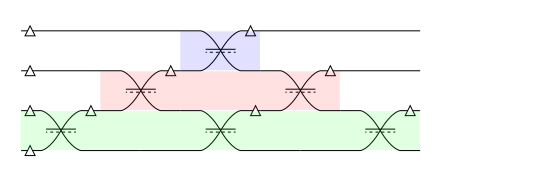
\includegraphics{figures/example}\\
  \vspace{5mm}
  \includegraphics[width=\columnwidth]{figures/graphs}
  \caption{A \(4 \by 4\) unitary, expressed in linear optics according to the
    scheme in \cite{re-prl-73-58}, and the appropriate \pdf{}s for choosing
    parameters for a Haar unitary. The reflectivities of the bottom three
    beamsplitters (region (a), shaded green) can be chosen uniformly from the
    interval \(\left[ 0,1 \right)\); those on the second row (region (b),
    shaded red) are chosen from a linear distribution biased towards lower
    reflectivities; and the top one is chosen from a quadratic distribution,
    even more biased towards lower reflectivities.}
  \label{fig:example}
\end{figure}
  
We have shown how to express the probability density function for Haar random
unitary matrices in terms of physically motivated parameters. The expression is
compact and non-redundant, whereas the equivalent in the Cartesian basis would
be a lot more complicated. While the mathematics of this process has been known
for a long time, the link to linear-optical components has not previously been
made clear, and the proof presented here in terms of a change of basis is much
simpler than that in \cite{sp-jpa-43-385306}. Our formula will have
applications in the emerging field of Boson Sampling, where photons are
injected into large Haar unitaries to demonstrate the power of quantum systems
over classical. Using the results contained here, the unitaries can be
generated directly in terms of the linear optical components without having to
go through the process of orthogonalising a Gaussian matrix.

\bibliography{bib/dialling}

\end{document}
